\documentclass[aps,prd,superscriptaddress,onecolumn,nofootinbib,preprintnumbers,notitlepage]{revtex4-1}
\usepackage[utf8]{inputenc}
\usepackage{amsmath,amssymb,mathtools}
\usepackage{tabularx}
\usepackage{siunitx}
% \usepackage{authblk}
% \usepackage{standalone}
\usepackage{xspace}
% \usepackage{hyperref}

\newcommand{\CM}{\mathrm{CM}}
\newcommand{\diff}{\mathrm{d}}
\newcommand{\chicO}{\ensuremath{\chi_{c1}}\xspace}


\begin{document}

\graphicspath{{../plots/}}

\title{$S$-matrix approach to the $\rho-\omega$ interference}
\author{Misha~Mikhasenko}\affiliation{CERN-EP, CH-1211, Geneva, Switzerland}\affiliation{JPAC}
\author{others}\affiliation{JPAC}

\begin{abstract}
  Amplitude of the $\rho/\omega$ interferece is constructed in $K$-matrix formalism.
Parameters of the scattering matrix are fixed using scattering phase shift and known partial width of the $\rho$,
  and $\omega$ mesons.
\end{abstract}

\nopagebreak
\maketitle

\section{Decay amplitude for $\chicO(3872)\to J/\psi \pi^+\pi^-$}
The process is described by a transition amplitude $M_{\lambda_0,\lambda_1}(m_{\pi^+\pi^-})$,
with $\lambda_0$ and $\lambda_1$ being the helicity of $\chicO$ and $J/\psi$.
The $\pi^+\pi^-$ system needs to be in $P$-wave with $J^{PC} = 1^{--}$ to give positive $C$ parity to $\chicO$.
The decay amplitude reads:
\begin{align}
  M_{\lambda_0,\lambda_1} = h_{\lambda_0+\lambda_1,\lambda_1} \,A_{\pi\pi}\,d_{\lambda_0+\lambda_1,0}^1(\theta_{\pi\pi})
\end{align}
where $A_{\pi\pi}$ is a the $\pi\pi$ production amplitude, $h$ is the helicity coupling.
The later simplifies in the LS basis since the parity and charge conjugation constraints can be enforced.
\begin{align}
  h_{\lambda_0+\lambda_1,\lambda_1} &= \sum_{S,L} \sqrt{\frac{2L+1}{3}}
    \left\langle 1,\lambda_0+\lambda_1;1,-\lambda_1 | S, \lambda_0\right\rangle
    \left\langle L 0;S, \lambda_0 | 1, \lambda_0\right\rangle h_{LS}\,q^L,\\
  % &= h_{S} + h_{D} q^2.
\end{align}
where we put explicit threshold factor $q^L$ with 
with $q = \lambda^{1/2}(m_{\chicO}^2,m_{J/\psi}^2,m_{\pi\pi}^2)$.
\footnote{We use the triangle function $\lambda(x,y,z) = x^2+y^2+z^2-2xy-2yz-2zx$.}
Due to the parity conservation only even waves are present.


Angular dependence vanishes once the decay in integrated
over the scattering angle $\theta_{\pi\pi}$. We also neglect $D$-wave in the $\chicO\to J\psi\rho$ decay.
\begin{align}
  I_{\pi\pi} \equiv \frac{\diff N}{\diff m_{\pi\pi}} &= p q \int \frac{\diff\cos\theta}{2} \sum_{\lambda_0,\lambda_1} | M_{\lambda_0,\lambda_1}|^2\\
  &= N\,p q \,|A_{\pi\pi}|^2.
\end{align}
where $p = \sqrt{s/4-m_\pi^2}$ is a pion break-up momentum,
$N$ is the overall normalization constant.

\section{Two-channels scattering}
We consider coupling between two channels:
\begin{itemize}
  \item $J^{PC}=1^{--}$: $\pi\pi\,P$-wave, and
  \item $J^{PC}=1^{--}$: $\rho\pi\,P$-wave.
\end{itemize}

First we factor out kinametic singularity related to the $P$-wave
\begin{equation}
  A_{\pi^+\pi^-} = \hat{A}_{\pi^+\pi^-} p, % B_1^{1/2}(p)
\end{equation}
% The production amplitude $A$ is calculated from the scattering matrix
% $B_1(p)$ is a threshold factor (+ barrier factor, e.g.\ the Blatt-Weisskopf function, $B_1(p) = p^2/(1+R^2p^2)$, $R=1.5/$GeV).
The scattering and production amplitudes are expressed through the $K$-matrix:
\begin{align} \label{eq:T.2x2}
  \hat{T} &= \left[1-i K \rho \right]^{-1} T\\
  \hat{A} &= \left[1-i K \rho \right]^{-1} N.
\end{align}
where $\rho$ is a diagonal matrix of the phase space elements with the square of the break-up momentum:
\begin{align}
  \rho_1(s) & = \frac{2p}{\sqrt{s}}\,\,B_1(p)\\
  \rho_2(s) & = \frac{1}{s} \int_{4m_\pi^2}^{(\sqrt{s}-m_\pi)^2} \frac{\diff \sigma}{2\pi \sigma}\,\,\frac{\lambda^{1/2}(s,\sigma,m_\pi^2) \lambda^{1/2}(\sigma,m_\pi^2,m_\pi^2)}{(m_\rho^2-\sigma)^2 + (m_\rho \Gamma_\rho)^2} B_1(p(\sigma)) B_1(k(\sigma)),
\end{align}
with $s\equiv m_{\pi\pi}$, 
$k(\sigma) = \lambda^{1/2}(s,\sigma,m_\pi^2)/(2\sqrt{s})$, and
$p(\sigma) = \lambda^{1/2}(\sigma,m_\pi^2,m_\pi^2)/(2\sqrt{\sigma})$.
The second expression represent a convolution of the two-body phase, $\rho^+\pi^-$\,$P$-wave with the lineshape of
the $\rho$ meson, $\rho\to\pi\pi$\,$P$-wave. We have neglected symmetrization of pions in the decay $\omega\to \pi^+\pi^-\pi^0$.

The $K$-matrix contains a pole at every channel and a small non-diagonal coupling between two channels.
\begin{equation} \label{eq:K}
  K = \frac{1}{m_1^2-s}\begin{pmatrix}
    g_1^2 & 0\\
    0 & 0
  \end{pmatrix} +
  \frac{1}{m_2^2-s}\begin{pmatrix}
    h_1^2 & h_1 h_2\\
    h_1 h_2 & h_2^2
  \end{pmatrix}
\end{equation}
The parameters of the $K$ matrix are completely fixed by the widths of the resonances and branching fractions:
\begin{align}
  g_1^2 & = m_\rho \Gamma_\rho / \rho_1(m_\rho^2),\\ \nonumber
  h_1^2 & = m_\omega \Gamma_\omega\,\text{Br}(\omega\to\pi^+\pi^-) / \rho_1(m_\omega^2),\\ \nonumber
  h_2^2 & = m_\omega \Gamma_\omega\,\text{Br}(\omega\to3\pi) / \rho_2(m_\omega^2).
\end{align}
We note that coefficient $h_1^2$ is extremely small compare to $g_2^2$.
\begin{figure}
  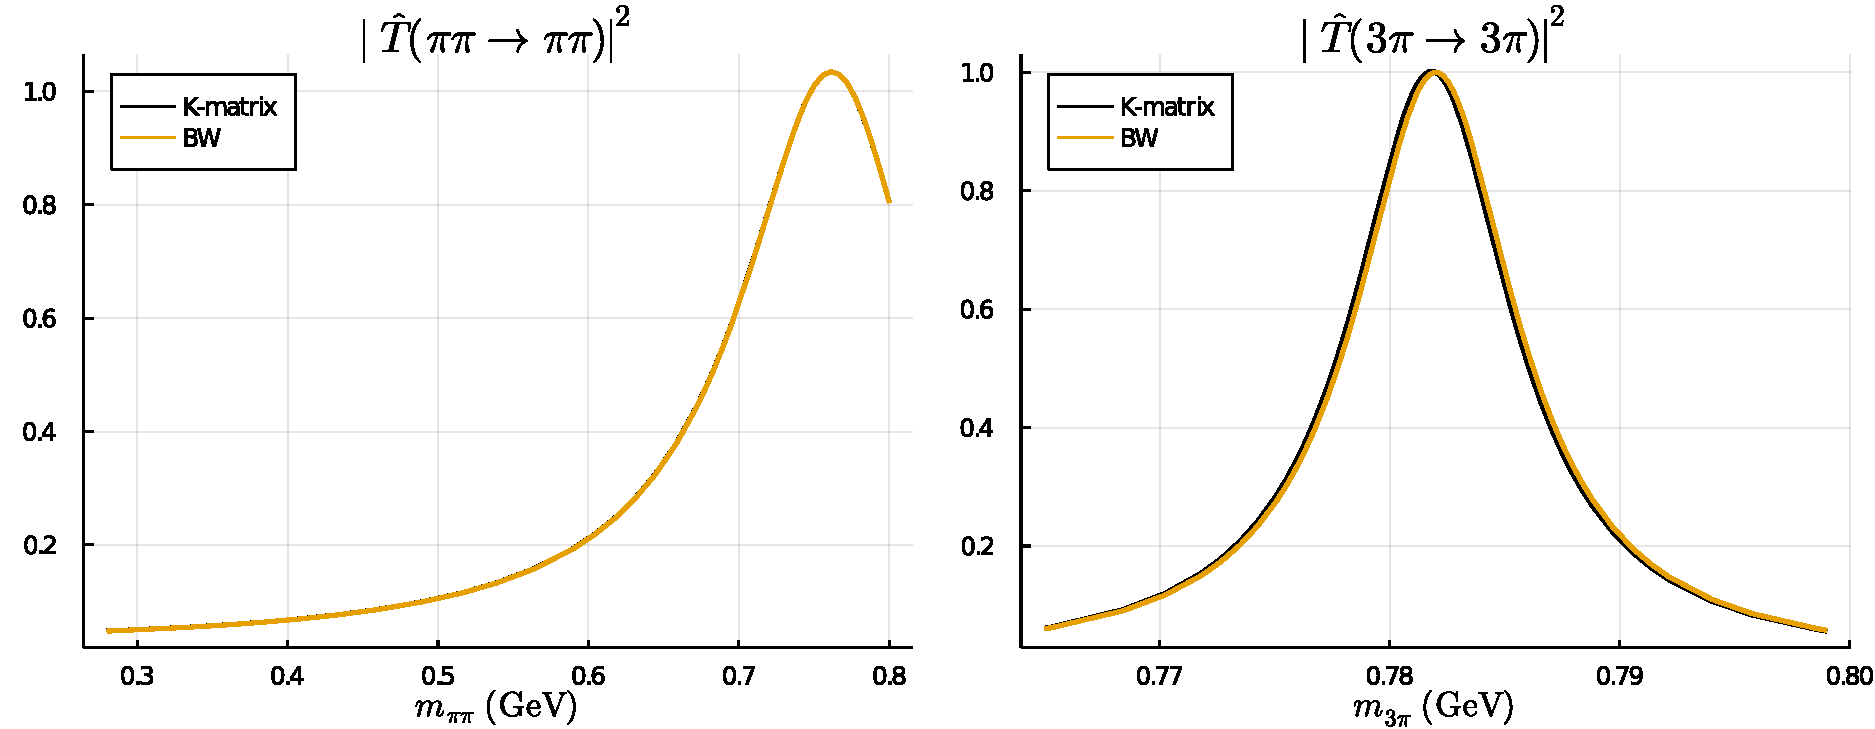
\includegraphics[width=0.9\textwidth]{BW_vs_Kmatrix.pdf}
  \caption{Diagonal terms of the $K$ matrix ampltude in comparison with the BW amplitde.}
\end{figure}


% The denominator of the scattering amplitude is proportional to the $\text{det}(\mathbb{I}-i K \rho)$.,
% that is a product of the $\rho$ and $\omega$ inverse propagators up to the terms proportional to $h_2^2$.
% \begin{align}
%   D & = (m_1^2-s)(m_2^2-s)^2\,\,\text{det}(\mathbb{I}-i\rho K) \\\nonumber
%     % & = h^{2} h_2^{2} \rho_{1} \rho_{2} (m_{1}^{2} - s) + \big(i \rho_{1}
%     % \left(g_{1}^{2} (m_{2}^{2} - s) + h^{2} (m_{1}^{2} - s)\right) \\\nonumber
%     % &\qquad - (m_{1}^{2} - s) (m_{2}^{2} - s)\big) \left(i h_2^{2} \rho_{2} - m_{2}^{2} + s\right)\\\nonumber
%     &= (m_1^2-s-ig_1^2\rho_1)(m_2^2-s-ih_2^2\rho_2)(m_2^2-s) + O(h_1^2).
% \end{align}

% We use the $Q$-vector approach for the construction of the production vector,
A general expression (Q and P vectors) for the production vector follow
\begin{equation}
  N = K\,[\alpha_1, \alpha_2]^T + [f_1, f_2]^T,
\end{equation}
where $\alpha_i$ and $f_i$ are constants.
the case $F = 0$ corresponds to the $Q$-vector approach.
% The terms we obtain an expression for the amplitude:
\begin{align} \label{eq:production}
\hat{A}_{\pi^+\pi^-} &= \alpha_{1} \hat{T}_{1,1} + \alpha_{2} \hat{T}_{1,2}.
\end{align}
Exlicitely,
\begin{align}
  \hat{A}_{\pi^+\pi^-} = \frac{
    \alpha_{1} \left(i h_{1}^{2} h_{2}^{2} \rho_{2} \left(m_{1}^{2} - s\right) -
    \left(g_{1}^{2} \left(m_{2}^{2} - s\right) + h_{1}^{2} \left(m_{1}^{2} - s\right)\right)
    \left(i h_{2}^{2} \rho_{2} - m_{2}^{2} + s\right)\right) +
    \alpha_{2} h_{1} h_{2} \left(m_{1}^{2} - s\right)
    \left(m_{2}^{2} - s\right)
  }{
    h_{1}^{2} h_{2}^{2} \rho_{1} \rho_{2} (m_{1}^{2} - s) +
  %
    \left(i \rho_{1} \left(g_{1}^{2} \left(m_{2}^{2} - s\right) + h_{1}^{2} \left(m_{1}^{2} - s\right)\right) -
    \left(m_{1}^{2} - s\right) \left(m_{2}^{2} - s\right)\right)
    %
    \left(i h_{2}^{2} \rho_{2} - m_{2}^{2} + s\right)}
\end{align}

When setting $h_1^2$ to zero, the amplitude becomes:
\begin{align}
  \left.\hat{A}_{\pi^+\pi^-}\right|_{h^2\to 0} = \frac{\alpha_1 g_1^2}{m_1^2 - s - i g_1^2 \rho_1} + \frac{\alpha_2 h_1 h_2 (m_1^2-s)}{(m_1^2 - s - i g_1^2 \rho_1)(m_2^2 - s - i h_2^2 \rho_2)}.
\end{align}
One finds an artificial zero at the second term originating from the $K$-matrix construction.
% It is later removed
% The $P$-vector appoach allows for additional freedom, the terms $(1-i\rho K)$
% \frac{- f_{1} g_{1}^{2} \left(i h_{2}^{2} ρ_{2} - m_{2}^{2} + s\right) + f_{2} h_{1} h_{2} \left(m_{1}^{2} - s\right)}{\left(i g_{1}^{2} ρ_{1} - m_{1}^{2} + s\right) \left(i h_{2}^{2} ρ_{2} - m_{2}^{2} + s\right)}
The zero is located at the value of the bare $\rho$ mass.
Since the bare mass does not have physical meaning and can be shifted arbitrary,
the zero does not need to be enforced there.
We remove it with the production coefficients:
\begin{align} \label{eq:production.poly}
  \alpha_1 &= \text{Pol}_m(s), & \alpha_2 &= \frac{\text{Pol}_n(s)}{m_1^2-s},
\end{align}
with $\text{Pol}_i(s)$ being a real polynomial of the order $i$.
One should be able to obtain a decent fit with $m=1$, $n=0$.
The higher order polynomials should be tried for systematic studies.
\begin{figure}
  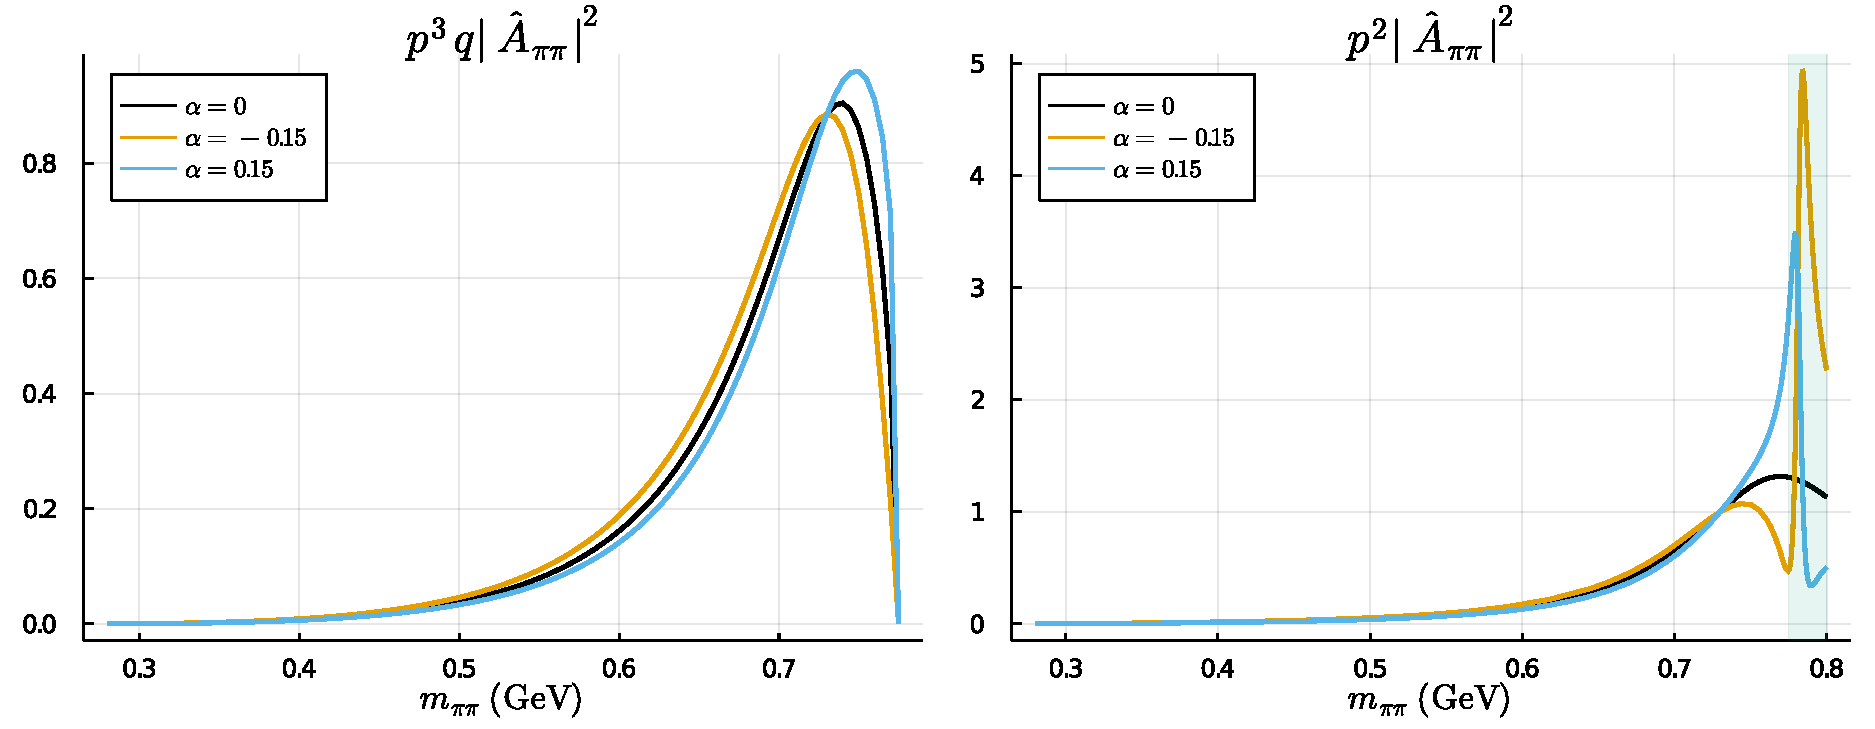
\includegraphics[width=0.9\textwidth]{X2pipi_intensity_combined.pdf}
  \caption{Two-pion production amplitude.
  The phase-space factor is removed on the light plot to highlight the region
  of large $\rho/\omega$ mixing.}
\end{figure}

% \section{Fit to the $e^{+}e^{-}$ data}

% The amplitudes $A^\rho$ and $A^{\rho/\omega}$ are given by the expressions:
% \begin{align}
%   A^\rho &= \frac{\left(g_{1}^{2} \left(m_{2}^{2} - s\right) + h^{2} \left(m_{1}^{2} - s\right)\right)
%     \left(m_{2}^{2} - s - i h_2^{2} \rho_{2}\right) + i h^{2} h_2^{2} \rho_{2} (m_{1}^{2} - s)}{D}
%     \nonumber &
%     = \frac{g_1^2}{m_1^2-s-ig_1^2\rho_1} + O(h_1^2) \\ \nonumber
%   A^{\rho/\omega} &= \frac{h_1 h_2 \left(m_{1}^{2} - s\right) \left(m_{2}^{2} - s\right)}{D} =
%   \frac{h_1 h_2 (m_1^2-s)}{(m_1^2-s-ig_1^2\rho_1)(m_2^2-s-ih_2^2\rho_2)} + O(h_1^2).
% \end{align}
% where we indicated a limit with $h\to 0$.

\section{A comment on $\omega\to\rho\pi$ phase space}
We compated several expressions that approximate $\rho\pi\,P$-wave
phase space factor in Fig.~\ref{fig:rhopi.ph.sp}.
\begin{figure}
  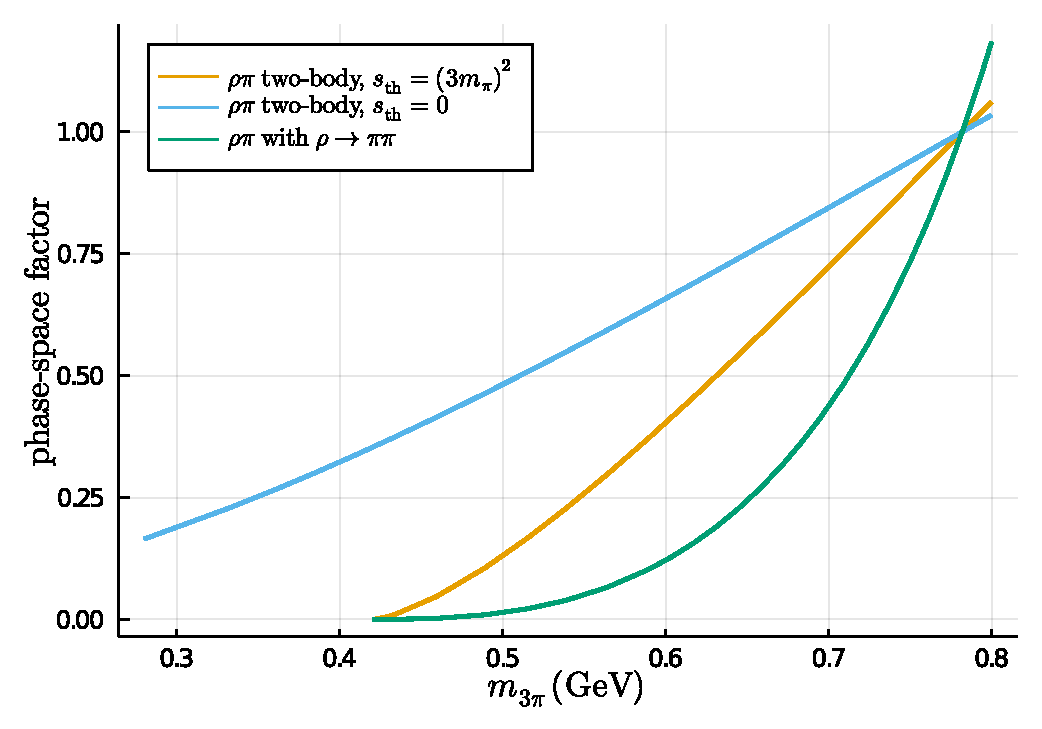
\includegraphics[width=0.46\textwidth]{phase_space_tb_vs_qtb.pdf}
  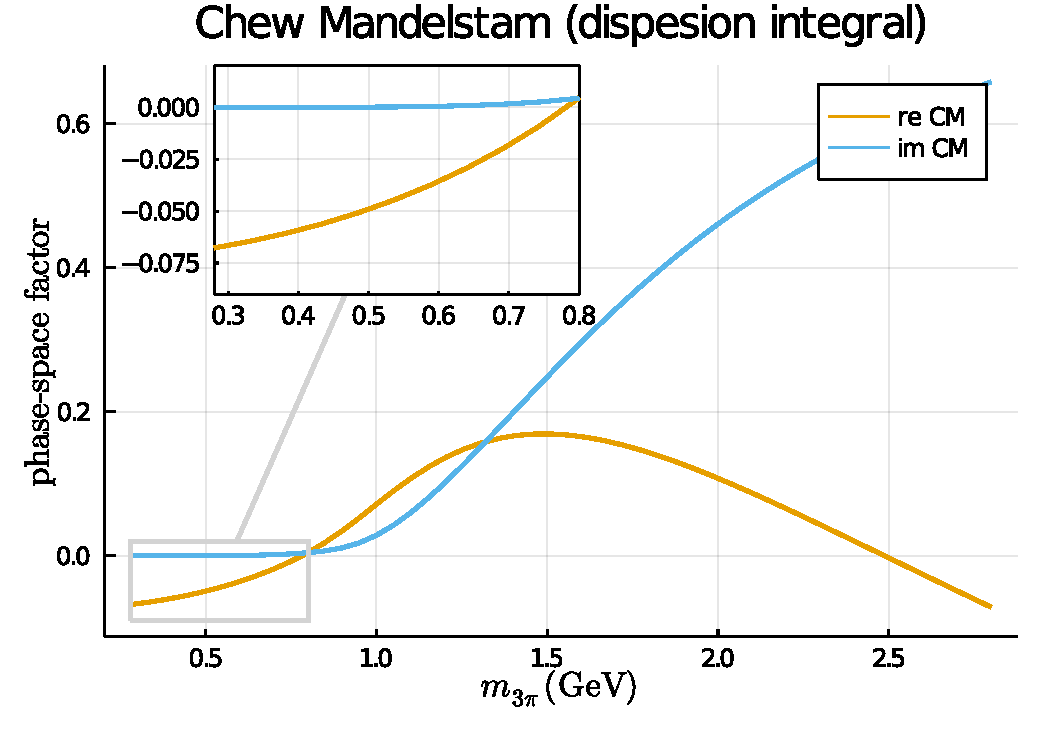
\includegraphics[width=0.46\textwidth]{qtb_dispersive_term.pdf}
  \caption{}
  \label{fig:rhopi.ph.sp}
\end{figure}
Due to the small width of $\omega$ the parametrization does not influence
the $\pi\pi$ amplitude.

% One can improve analytic structure of the amplitude by replacing the phase-space factors
% by their dispersive representation:
% \begin{equation} \label{eq:CM}
% i\rho_i \to (\CM_i - \text{Re}\,\CM_i(m_i^2)), \quad
% \CM_i = \frac{s}{\pi}\int_{4m_\pi^2}^{\infty} \frac{\diff s'\,\rho_i(s')}{s'(s'-s-i\epsilon)}
% \end{equation}

% Instread of using a constant for the expression for the $\rho\pi\,P$-wave,
% the quasi-two-body phase space can be calculated:
% \begin{equation}
% \rho_2 \to \frac{1}{s} \int_{4m_\pi^2}^{(\sqrt{s}-m_\pi)^2} \frac{\diff \sigma}{2\pi \sigma}\,\,\frac{\lambda^{1/2}(s,\sigma,m_\pi^2) \lambda^{1/2}(\sigma,m_\pi^2,m_\pi^2)}{(m_\rho^2-\sigma)^2 + (m_\rho \Gamma_\rho)^2} B_1(k) B_1(q),
% \end{equation}
% \begin{equation}
%   K = \frac{1}{m_1^2-s}\begin{pmatrix}
%     g_{13}^2 & 0\\
%     0 & 0
%   \end{pmatrix} +
%   \frac{1}{m_2^2-s}\begin{pmatrix}
%     g_{14}^2 & g_{14} g_{24}\\
%     g_{14} g_{24} & g_{24}^2
%   \end{pmatrix}
% \end{equation}

\section{Matching the amplitude to known $\pi^+\pi^-$ phase shifts}
In this section we address contribution of $\rho(1450)$ and $F$-wave
and argue that for the region of $m_{\pi^+\pi^-}$ below $0.8\,$GeV these contributions
are irrelevant. $\pi^+\pi^-\,P$-wave is essentially elastic below $1\,$GeV,
therefore the scattering/production amplitudes are proportional
to the sine of the scattering phase $\delta_1$.
These scattering phases are well established, e.g. in analysis of the Madrid group~\cite{GarciaMartin:2011cn}.
Fig.~\ref{fig:scatt.phases} shows the phase of the $F$-wave as well as the phase
of $P$-wave in several models. The $F$-wave reaches just $0.25\,$deg. at $m_{\pi^+\pi^-}^{(\text{max})}=0.8\,$GeV. compare to $108.65\,$deg. of $P$-wave.
It gives three order of magnitude suppression of the $F$-wave amplitude if the same production strength is used for both waves.
\begin{figure}
  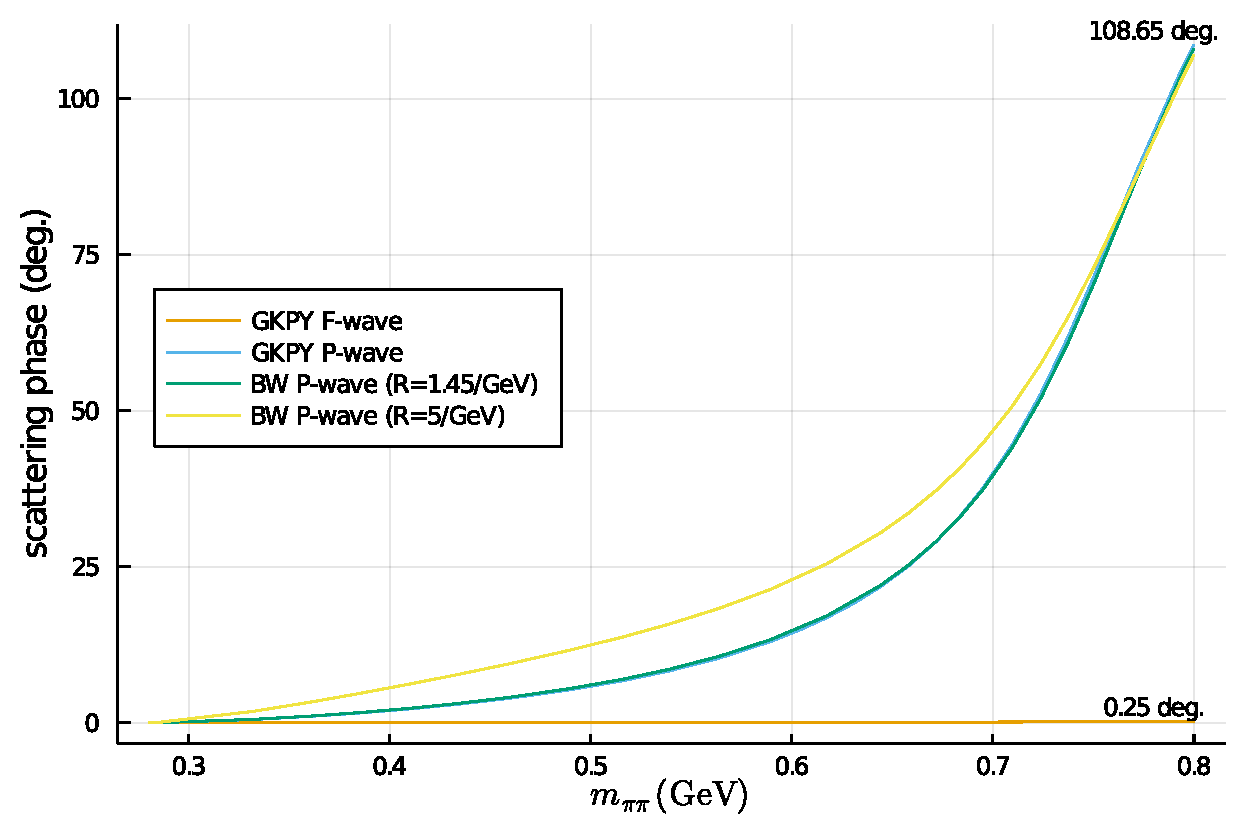
\includegraphics[width=0.7\textwidth]{Pwave_phaseshift.pdf}
  \caption{The $\pi^+\pi^-$ P-wave and F-wave scattering phases from the phenomenological analysis of Ref.~\cite{GarciaMartin:2011cn} and the single-pole amplitude with CM function.
  Note that the green line is right on top of the blue line with a little deviation at the limit of the phase space.}
  \label{fig:scatt.phases}
\end{figure}
The phase shift of the $P$-wave for the standard Breit-Wigner amplitude to the one extracted from phenomenological analysis~\cite{GarciaMartin:2011cn} shows a large difference (compare yellow curve and the blue curve)
The difference almost vanishes once the size parameter $R$ is tuned to $1.4/$GeV.
The value of this parameter in the range from $1.3$ to $1.5$ gives the phase shift bearely distringuishable from the Madrid $\pi\pi$ phase shift.
% The Chew-Mandelstam function,
% Eq.~\eqref{eq:CM} is used for the energy-dependent width.
% The further difference between the Madrid phase (orange line) shows and the adjusted curve
% shows potential contributions of the other poles, i.e. $\rho'(1450)$.

\newpage

\appendix

\section{Altermative formulations}
The amplitude can be written in the other form:
\begin{align} \label{eq:T4x4}
  T = G\,\Sigma\,G\,\Sigma\,G\,\Sigma\,G\dots = (1- G \Sigma)^{-1} G,
\end{align}
where $\Sigma$ and $G$ are $4\times 4$ matrices
\begin{align}
  G &=
  \begin{pmatrix}0 & 0 & g_{13} & g_{14}\\0 & 0 & 0 & g_{24}\\g_{13} & 0 & 0 & 0\\g_{14} & g_{24} & 0 & 0\end{pmatrix},&
  \Sigma &=
  \begin{pmatrix}
    i\rho_1 & 0 & 0 & 0\\
     0 & i\rho_2 & 0 & 0\\
     0 & 0 & \frac{1}{m_1^2-s} & 0\\
     0 & 0 & 0 & \frac{1}{m_2^2-s}.
  \end{pmatrix},
\end{align}
i.e. $G$ is a matrix of coupligns, $\Sigma$ is either particle propagator, or a particle loop.
The coupling matrix makes sure that the particle propagator,
and a particle loop are always interchange (only element at the off-diagonal $2\times 2$ blocks are allowed).

The production amplitude has the form:
\begin{align} \label{eq:A4.production}
  \hat{A}_{\pi^+\pi^-} = \sum_{i=1}^4 T_{1,i} \alpha_i
\end{align}

The submatrix $T_{(1,2),(1,2)}$ in Eq.~\eqref{eq:T4x4} it is exactly equal to Eq.~\eqref{eq:T.2x2},
with the following correspondence in Eq.~\eqref{eq:K},
\begin{align}
  g_{13} &\Rightarrow g_1,&
  g_{14} &\Rightarrow h_1,&
  g_{24} &\Rightarrow h_2.
\end{align}
Hence, the $T_{1,1}\alpha_1 + T_{1,2}\alpha_2$ is exactly equal to the sum in Eq.\eqref{eq:production}.

To identify the terms $T_{1,3}$ and $T_{1,4}$ in Eq.~\eqref{eq:A4.production} further,
we show explicit expressions for $T_{1,i}$ in the limit $g{14}^2 \to 0$:
\begin{align}
  \hat{T}_{1,1} &= \frac{g_{13}^2}{m_\rho^2-s-ig_{13}^2 \rho_1}\\
  \hat{T}_{1,2} &= \frac{g_{14} g_{24} (m_\rho^2-s)}{(m_\rho^2-s-ig_{13}^2 \rho_1)(m_\omega^2-s-ig_{24}^2 \rho_2)}\\
  \hat{T}_{1,3} &= \frac{g_{13}^2 (m_\rho^2-s)}{m_\rho^2-s-ig_{13}^2 \rho_1}\\
  \hat{T}_{1,4} &= \frac{g_{14} (m_\rho^2-s)(m_\omega^2-s)}{(m_\rho^2-s-ig_{13}^2 \rho_1)(m_\omega^2-s-ig_{24}^2 \rho_2)}.
\end{align}
Both terms, $\hat{T}_{1,3}$ and $\hat{T}_{1,3}$ have artificial zeros $(m_\rho-s)$ or/and $(m_\rho-s)$ in the numerators.
If we cancel this zero by a pole in the production vector as we did in Eq.~\ref{eq:production.poly},
these terms becomes the same as $T_{1,1}$ and $T_{1,2}$.
If only $(m_1^2-s)$ term suppressed in $T_{1,2}$ and $T_{1,4}$,
adding $T_{1,3}\alpha_3$ and $T_{1,4}\alpha_4$ is equivalent of using $\text{Pol}_1$ in Eq.~\ref{eq:production.poly}.

% \section{Other check with different production amplitude}
% $P$-vector production gives more flexible parametrization
% \begin{equation}
%   N_i = \sum_R \left( \frac{\alpha_i^R}{m_R^2-s} + f_i \right).
% \end{equation}
% With an assumption that direct decay of $X$ to $J/\psi\,3\pi$ is negligible, i.e. $f_2 = 0$, we get:
% \begin{align}
%   \hat{A}_{\pi^+\pi^-} &=
%     \frac{1}{m_1^2-s-ig_1^2\rho_1} \left(
%     \alpha_1^{\rho} + \frac{k \alpha_2^\omega (i\rho_2) (m_1^2-s)}{(m_2^2-s-ih_2^2\rho_2)(m_2^2-s)}
%   \right)  + \frac{f_1(m_1^2-s)}{m_1^2-s-ig_1^2\rho_1}\\\nonumber
%   &=
%     \frac{1}{m_1^2-s-ig_1^2\rho_1} \left(
%     \alpha_1^{\rho\prime} + \frac{k \alpha_2^\omega (m_1^2-s)}{m_2^2-s-ih_2^2\rho_2}
%   \right)  + \frac{f_1(m_1^2-s)}{m_1^2-s-ig_1^2\rho_1}
% \end{align}

% \subsection{The final reasonable forms}
% We find that unitality-guided amplitude contains two type of terms:
% $\rho$-term and $\rho\times\omega$-term with, in principle, arbitrary numerator functions.
% The pragmatic approach would be to leave freedom adjust $\rho$-meson lineshape
% at the full range of spectrum and allow for local modification in vicinity of the $\omega$ mass.
% \begin{align}
%   \hat{A}_{\pi^+\pi^-}
%   & = \frac{c^{\rho} + c^{\pi^+\pi^-}(m_1^2-s)}{m_1^2-s-ig_1^2\rho_1}
%    + \frac{c^{\rho}}{(m_2^2-s-ih_2^2\rho_2)(m_1^2-s-ig_1^2\rho_1)}\\
%   \mathrm{OR,} & =
%   \frac{a + bs}{m_1^2-s-ig_1^2\rho_1}\left(
%     1+ \frac{c}{m_2^2-s-ih_2^2\rho_2}
%   \right).
% \end{align}


\bibliographystyle{apsrev4-1}
\bibliography{rho_omega}
\end{document}
